\chapter{Discussion}

We have shown that our approach is capable of generally improving F1-scores in Widar 3.0, but our overall performance is disappointing, compared to both baselines and state-of-the-art approaches.
In this chapter, we discuss the experimental results and what these results mean with respect to our research questions, analyze the latent space and domain embeddings produced by our approach, as well as suggest future research that may be taken.

\section{Comparison to State-of-the-Art}

\begin{figure}
	\centering
	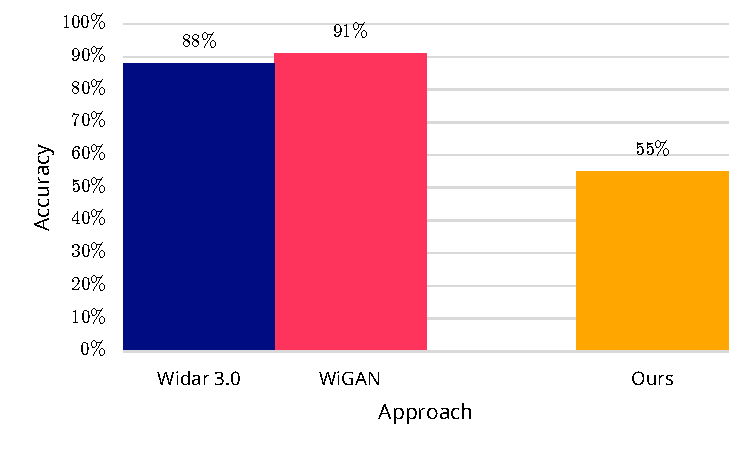
\includegraphics[width=5in]{figures/results_sota}
	\caption{Comparison of our method against the Widar 3.0 benchmark and the current SOTA. The space between our work and other works is intentionally placed to reiterate the point that these values are not directly comparable as our data splits, although both representing single-user leave-out, are not comparable.}
	\label{fig:results-sota}
\end{figure}

It is difficult to compare our results to the state-of-the-art (SOTA), as we do not train on the same training splits as those SOTA models.
We can, though, make a rough comparison to the CNN baseline in the Widar 3.0 paper \cite{zheng2019zero} and to the WiGAN approach in \cite{jiang2020wigan}.
Both these papers provide results for single-user leave-out and the performance comparison with our method can be seen in Figure \ref{fig:results-sota}.
In Widar 3.0, the CNN approach used is able to provide a baseline result of $88\%$ accuracy in single-user leave-out while 
WiGAN is able to achieve $91\%$ accuracy.
These methods both provide significantly better results than DARLInG, which achieves a best performance of $49\%$ accuracy when using DDPG with MTF.

It should be reiterated, though, that these numbers are not directly comparable as they do not use the same dataset splits.

\section{Research questions}

In this section, we answer each of the research questions we posited in Section \ref{sec:intro-problem-statement} as well as a short discussion on the strengths and limitations of our approach to answering these questions.

\paragraph{Research Question 1}
Our first question asks how well DARLInG's embed heads perform compared to its null heads.
The results from Section \ref{sec:experiments-setup-results} show that using an RL agent indeed has the potential to increase out-of-domain performance by up to 6.2 percentage points but may also provide no benefit.
Using MTF as the transform, DDPG as the RL agent, and one-hot encoding as the domain embedding encoding provides our best results, but its low performance with the two other transforms suggest that this may not always be the case.
As such, we can conclude that while not very satisfying, our results suggest that using RL to provide unsupervised domain labels \textit{may} provide better out-of-domain performance on Widar 3.0.

\paragraph{Research Question 2}
Our second question asks how changing the domain embedding encoding affects performance.
Generally, we see inconclusive results with both encodings providing no meaningful difference generally while providing some difference with DDPG with MTF and RP transforms.
Even in these two cases, though, the difference is inconclusive as MTF prefers one-hot encoding while RP prefers probability measure encoding.
As a result, we believe that the domain embedding is not significant and that other factors contribute more towards the performance of the model.
Further research may be necessary to investigate the optimal encoding of the domain embedding.

\paragraph{Research Question 3}
Our last research question asks how changing the signal-to-image transformation affects performance.
Our results indicate that generally, GAF performs consistently, but not impressively.
MTF seems to perform quite well with DDPG and similarly to GAF with PPO.
RP seems to perform poorly with PPO, not improving over the null head, while performing similarly to MTF with DDPG.
As a result, we can confidently conclude that different signal-to-image transformations affect model performance, but the results are inconclusive as to which transformation works best.
The results do suggest, though, that MTF may be the best performer in our experiments of limited sample size.

\paragraph{Strengths and Limitations}
We believe that our experiments are quite thorough with significant resources put into ensuring that the model itself is working appropriately, as well as that the code is free of any significant bugs which could render the results invalid.
Significant effort was put into ensuring that every step of the CSI processing and transformation pipeline produced the correct results during the course of writing the thesis.
The VAE was also checked by running the VAE with the Fashion-MNIST dataset \cite{xiao2017fashion}.
This produced results as expected with the VAE being able to adequately reconstruct the input images as well as classify the images appropriately with $>0.85$ accuracy, matching the benchmarks in \cite{xiao2017fashion}.
Finally, the RL algorithms used are off-the-shelf implementations from stable-baselines3 implemented according to the sample code provided, reducing the likelihood of programmatic issues with the RL algorithms.

Limitations include reduced hyperparameter tuning and the reduced training time of the RL agents.
RL agents are notoriously time-consuming to train \cite{schulman2017proximal,schulman2017trust,lillicrap2015continuous}.
With our limited compute resources, namely a laptop and a PC, we were unable to conduct a full hyperparameter optimization sweep of the RL agents.
We mostly used known good hyperparameters when dealing with a continuous action space for our agents.
Additionally, we were only able to train for a fraction of the time usually used to train RL agents.
We also approached a PhD candidate at the TU/e specializing in RL who concurred with our ideas on the alternating training style, where we iterate between training the RL agent and the VAE \cite{grooten2023interview}.

\section{Latent Space and Domain Embedding analysis}\label{sec:discussion-ls-de-analysis}

\begin{figure}
	\centering
	\begin{subfigure}{0.3\textwidth}
		\centering
		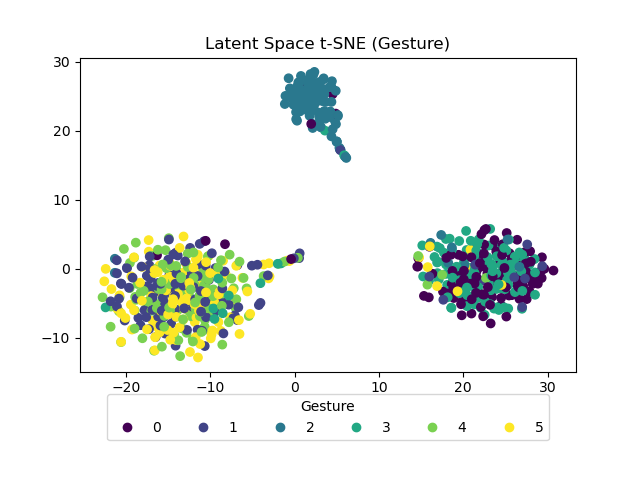
\includegraphics[width=\textwidth]{figures/mtf-ppo-one/ls-gesture}
		\caption{t-SNE by gesture}
		\label{fig:mtf-ppo-one-ls-gesture}
	\end{subfigure}
	\hfill
	\begin{subfigure}{0.3\textwidth}
		\centering
		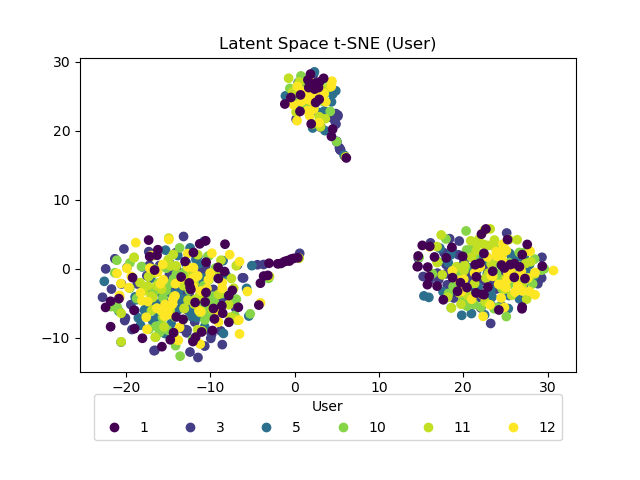
\includegraphics[width=\textwidth]{figures/mtf-ppo-one/ls-user}
		\caption{t-SNE by user}
		\label{fig:mtf-ppo-one-ls-user}
	\end{subfigure}
	\hfill
	\begin{subfigure}{0.3\textwidth}
		\centering
		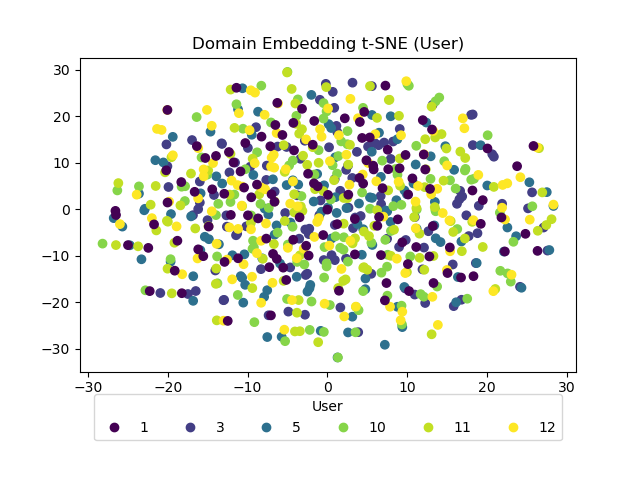
\includegraphics[width=\textwidth]{figures/mtf-ppo-one/de-user}
		\caption{t-SNE by User}
		\label{fig:mtf-ppo-one-de-user}
	\end{subfigure}
	\caption{t-SNEs of the latent space and domain embeddings produced by PPO with one-hot encoding and MTF transformation}
	\label{fig:mtf-ppo-one}
\end{figure}
\begin{figure}
	\centering
	\begin{subfigure}{0.3\textwidth}
		\centering
		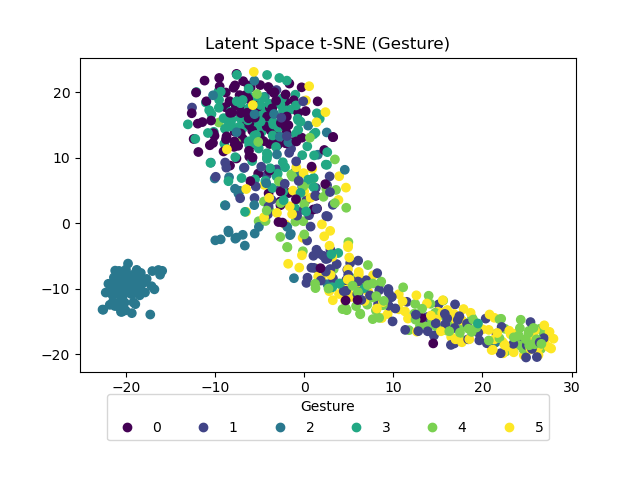
\includegraphics[width=\textwidth]{figures/mtf-ppo-pm/ls-gesture}
		\caption{t-SNE by gesture}
		\label{fig:mtf-ppo-pm-ls-gesture}
	\end{subfigure}
	\hfill
	\begin{subfigure}{0.3\textwidth}
		\centering
		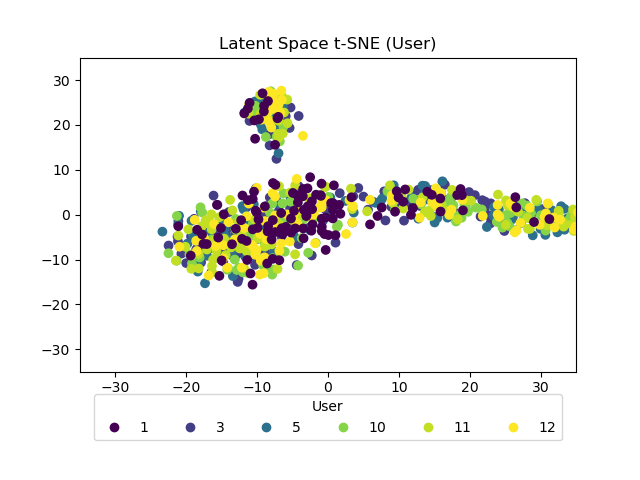
\includegraphics[width=\textwidth]{figures/mtf-ppo-pm/ls-user}
		\caption{t-SNE by user}
		\label{fig:mtf-ppo-pm-ls-user}
	\end{subfigure}
	\hfill
	\begin{subfigure}{0.3\textwidth}
		\centering
		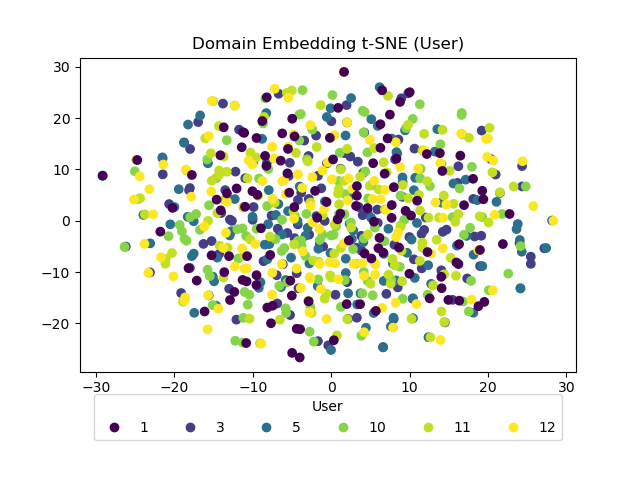
\includegraphics[width=\textwidth]{figures/mtf-ppo-pm/de-user}
		\caption{t-SNE by user}
		\label{fig:mtf-ppo-pm-de-user}
	\end{subfigure}
	\caption{t-SNEs of the latent space and domain embeddings produced by PPO with one-hot encoding and MTF transformation}
	\label{fig:mtf-ppo-pm}
\end{figure}

To properly analyze the low performance of our model, we would like to analyze both the latent space $\boldsymbol{z}$ produced by our encoder as well as the domain embeddings $\boldsymbol{d}_{r}$ produced by our RL agent.
We do this by running the entire dataset through both the encoder and RL agent and take the outputs and produce t-SNE embeddings out of these outputs.
By doing so, we can see if there is any structure to the embeddings.
We specifically analyze the case of using MTF as the signal-to-image transformation, PPO as the agent, and both the one-hot and probability measure domain embedding encodings, the results of which can be seen in Figures \ref{fig:mtf-ppo-one} and \ref{fig:mtf-ppo-pm}.

We can see that for the latent space, in both cases there is a much clearer structure, especially with gesture 2 being separated out quite distinctly in both Figures \ref{fig:mtf-ppo-one-ls-gesture} and \ref{fig:mtf-ppo-pm-ls-gesture}. 
Interestingly, both Figures \ref{fig:mtf-ppo-one-ls-user} and \ref{fig:mtf-ppo-pm-de-user} show quite an even distribution of users throughout each cluster in the t-SNE space.

For the domain embeddings, we see that there is \textit{some} structure in Figures \ref{fig:mtf-ppo-one-de-user} and \ref{fig:mtf-ppo-pm-de-user}, as it is not only a single normally-distributed disk, but there is not much of it.
We also see that the users, including the single-leave out user (user 1) is distributed quite evenly throughout the space in both figures.
This suggests that the RL agent is not able to accurately provide significantly different domain embeddings between the users.
We believe this may be simply due to training time constraints.

\begin{figure}
	\centering
	\begin{subfigure}{0.3\textwidth}
		\centering
		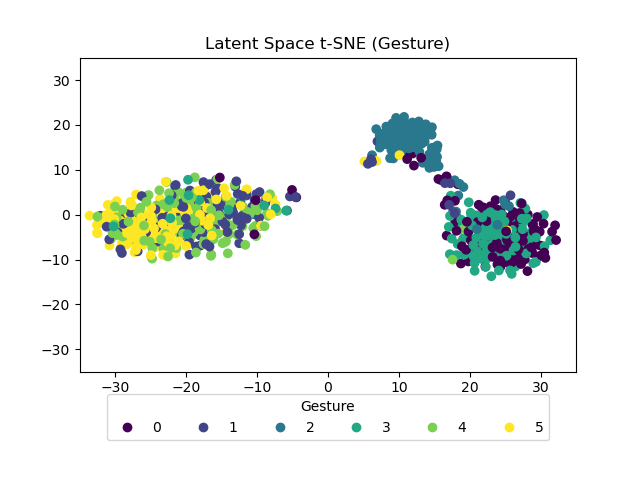
\includegraphics[width=\textwidth]{figures/extended/long_ls_gesture}
		\caption{t-SNE by gesture}
		\label{fig:extended-ls-gesture}
	\end{subfigure}
	\hfill
	\begin{subfigure}{0.3\textwidth}
		\centering
		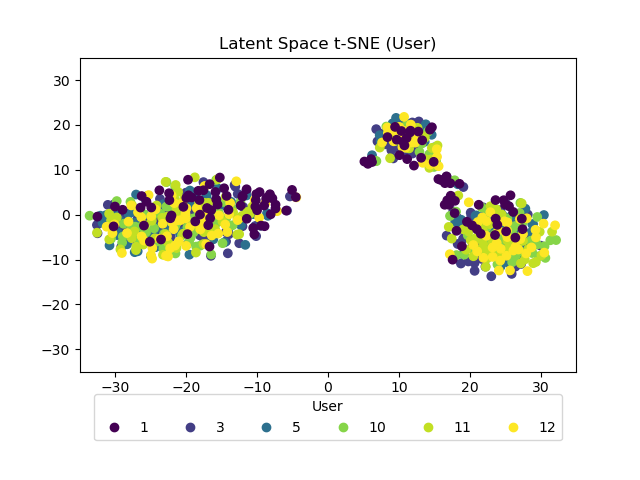
\includegraphics[width=\textwidth]{figures/extended/long_ls_user}
		\caption{t-SNE by user}
		\label{fig:extended-ls-user}
	\end{subfigure}
	\hfill
	\begin{subfigure}{0.3\textwidth}
		\centering
		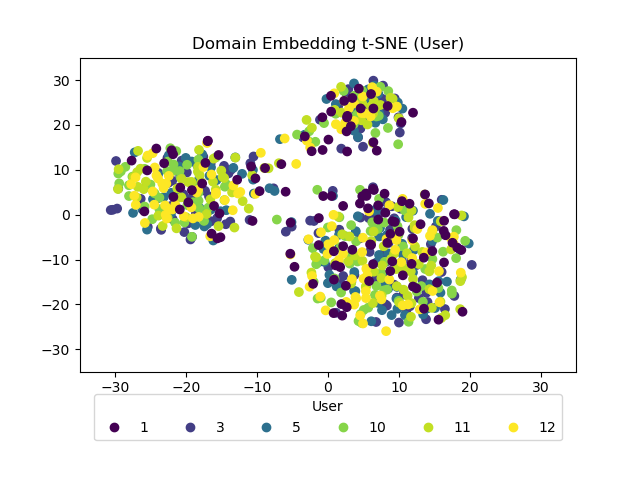
\includegraphics[width=\textwidth]{figures/extended/long_de_user}
		\caption{t-SNE by user}
		\label{fig:extended-de-user}
	\end{subfigure}
	\hfill
	\begin{subfigure}{0.3\textwidth}
		\centering
		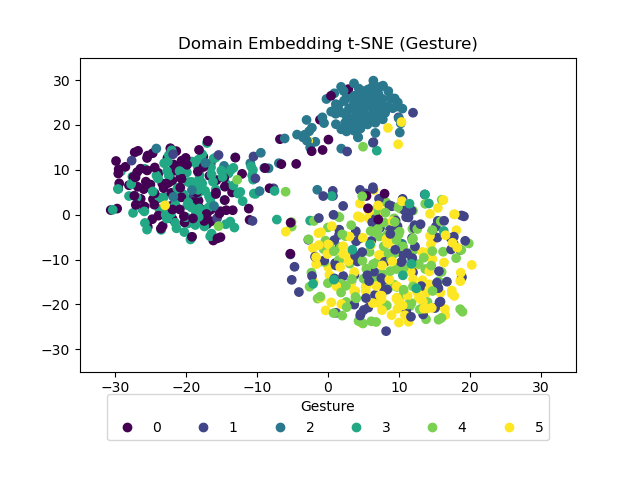
\includegraphics[width=\textwidth]{figures/extended/long_de_gesture}
		\caption{t-SNE by gesture}
		\label{fig:extended-de-gesture}
	\end{subfigure}
	\hfill
	\caption{t-SNEs of the latent space and domain embeddings produced by PPO with one-hot encoding and MTF transformation with extended training time.}
	\label{fig:extended-tsnes}
\end{figure}

To test this hypothesis, we trained our agent for longer, as was described in Subsection \ref{subsec:experiments-longer}.
The t-SNEs of this run can be seen in Figure \ref{fig:extended-tsnes}.
We notice that 

To analyze this further, we filtered the both the latent space and domain embedding t-SNEs by user and colored by gesture to see if the users have distinct structures or patterns in either the t-SNE plots.
We notice some clearer separation by gesture in Figure \ref{fig:extended-ls-gesture}, with gestures 2 and 0 being more clearly separated on the right side clusters.
Additionally, Figure \ref{fig:extended-ls-user} shows some more clustering within clusters for the users. For example, user 1 is primarily clustered towards to the top of the left-side cluster, for example.
Finally, we finally see some structure brought to the domain embeddings, with 3 clearly visible clusters in Figure \ref{fig:extended-de-user}, although they do not seem to correspond to the users themselves.

We additionally plotted the domain embedding t-SNE colored by gesture in Figure \ref{fig:extended-de-gesture}, and we notice that the domain embeddings are instead clustered by gesture.
This is interesting, as it means that our domain embeddings are in fact directly providing data on the gesture for the embed head, instead of simply providing data about the domain.
This would imply that we have some sort of meta-model made up of the embed head and the RL agent which together attempt to provide better gesture classifications.
We also plotted the domain-embedding t-SNE colored by gesture for the both other configurations, but we see no such clustering in those and as such, for brevity, will not include the plots.

We also plotted the latent-space and domain embedding t-SNEs, filtered by user and colored by gesture to analyze whether this provides any additional insight.
After analyzing these plots, we do not see any additional insight that can be taken from them, but nonetheless they are available in Appendix

\section{Future Research}

We believe that there may still be potential in our approach.
Further research could be aimed at a different neural-network architecture, hyperparameter tuning of the RL agents and some changes to the training regime.

\subsection{A Different Architecture}

Although our preliminary experiments in Section \ref{sec:experiments-preliminary} suggested that our VAE model could perform adequately for the task of gesture classification with the Widar 3.0 dataset, it was evidently not up to the task of gesture classification where the input is domain shifted.
One may, instead of using a VAE, use one of the known performant models from Section \ref{sec:literature-csi-for-gesture}.
This may result in better cross-domain performance to begin with with our RL approach adding the few percentage-points on top to make said models competitive with single-domain models.

\subsection{Hyperparameter Tuning of the RL Agent}

Due to time constraints, we conducted little hyperparameter tuning of the RL agent due to time and compute constraints. 
Future research may simply repeat our experiments but with increased time and  constraints to see if that could help at all.

We might also develop a different reward function which forces the agent to provide a domain embedding which more clearly provides additional information about the domain itself, instead of additional information about the gesture as our agent seems to have done as seen in the analysis in Section \ref{sec:discussion-ls-de-analysis}.

\subsection{A Different Training Regime}

Finally, we see in the loss curves of our experiments that there is a always a sudden increase in the loss function of the model, with a corresponding drop of around 0.05—0.10 in validation accuracy of the null head, at the epoch in which we introduce the embed head.
This decrease in validation accuracy of the null head may indicate that the changes our model makes to the latent space while trying to optimize for the embed head and RL agent is adversely affecting the performance of the null head.
Put another way, the null head is not capable of adapting to the changes in the latent space which the model makes while trying to optimize for the embed head.
We suggest that future work could look into two different approaches to this problem: By training the embed head iteratively on a frozen encoder and null head and the embed head only, or by changing the way we introduce the embed head using a process we propose called Simulated Aging and Hardening.

It might be possible to reduce the decrease in performance of the null head, and potentially increase overall performance, by training the embed head as an entirely separate network to the encoder and null heads.
In this approach, during the VAE training portion of every epoch, the encoder and null head would first be trained over the entire training set.
After every batch has been processed and the optimizers run for the encoder and null head, the parameters of said modules would be frozen.
At this point, we will start optimization on the embed head.
The same training set will be run through the encoder again and the produced outputs $\boldsymbol{z}$ along with the produced domain embeddings $\boldsymbol{d}_r$ from the RL agent (also frozen) would be run through the embed head to produce its gesture class predictions.
This would ensure that the embed head is being trained to predict only based on the $\boldsymbol{z}$ and $\boldsymbol{d}_r$ without affecting the encoder or the null head.
By doing so, the RL agent is forced to learn from an environment which is not itself adapting to the actions of the agent, potentially simplifying the environment evolution for the agent.

We might also attempt to instead slowly increase the rate of optimization of the embed head in a process we propose to be called \textit{Simulated Aging and Hardening} (SAH), directly inspired by the analogy used by simulated annealing (SA) to metallurgy.
In SA, we use an initial solution and explore neighboring solutions. 
Over time, we slowly ``cool down'' the probability of accepting worse solutions until we arrive at a near-optimal solution.
In this way, SA can be said to start of very exploratory and slowly reduce its exploration and increase its exploitation of known good solutions.
Conversely, our proposed SAH follows the process of aging and hardening, which is the opposite process in metallurgy.
The steps to hardening in metallurgy is typically as follows: Start with a metal that is at a high temperature, quench it to rapidly cool it down ``freezing'' the allowing elements in the metal, and finally slowly heat up the metal in a process called aging and hardening.

In SAH, applied directly to our use case, we would train the encoder and null heads in the same way we do now until the epoch where the embed head and RL agent starts training.
At this point, we would freeze the training of the encoder and null heads and optimize for only the embed agent, which is a duplicate of the null head with duplicated parameters
We do this with a lower learning rate than before
This is done so that the embed head will take smaller steps towards the new minima with the domain embedding from the RL agent.
After a certain number of epochs, or some heuristic is reached, we then continue training the model as a whole with the current training method described in this thesis.